% 注意事项:编译两次,以确保目录、页码完整显示

\def\allfiles{}

\documentclass[14pt,a4paper,UTF8,twoside]{article}

% Formatting Packages ——————————————————————————————————————
\usepackage{multicol}
\usepackage{multirow}
\usepackage{enumitem}
\usepackage{indentfirst}
\usepackage[toc]{multitoc}

% Math & Physics Packages ————————————————————————————
\usepackage{amsmath, amsthm, amsfonts, amssymb}
\usepackage{setspace}
\usepackage{physics}
\usepackage{cancel}
\usepackage{nicefrac}
\usepackage{unicode-math} % 允许数学公式使用特定字体

% Image-related Packages —————————————————————————————
\usepackage{float} % 浮动体环境
\usepackage{subcaption} % 子图包
\usepackage{graphics, graphicx}
\usepackage{tikz, tikz-qtree}
\usetikzlibrary{arrows.meta}
\usepackage{pgfplots}
\pgfplotsset{compat=1.18}
\usepackage{xcolor}
\usepackage{fourier-orns}
\usepackage{lipsum}
\usetikzlibrary{arrows.meta} % 加载arrows.meta库

% Colour Palette ——————————————————————————————————————
\definecolor{merah}{HTML}{F4564E}
\definecolor{merahtua}{HTML}{89313E}
\definecolor{biru}{HTML}{60BBE5}
\definecolor{birutua}{HTML}{412F66}
\definecolor{hijau}{HTML}{59CC78}
\definecolor{hijautua}{HTML}{366D5B}
\definecolor{kuning}{HTML}{FFD56B}
\definecolor{jingga}{HTML}{FBA15F}
\definecolor{ungu}{HTML}{8C5FBF}
\definecolor{lavender}{HTML}{CBA5E8}
\definecolor{merjamb}{HTML}{FFB6E0}
\definecolor{mygray}{HTML}{E6E6E6}
\definecolor{mygreen}{rgb}{0,0.6,0}
\definecolor{mymauve}{rgb}{0.58,0,0.82}

% Theorems ————————————————————————————————————————————
\usepackage{tcolorbox}
\usepackage{changepage}
\tcbuselibrary{skins,breakable,theorems}

\newcounter{hitung}
\setcounter{hitung}{\thesection}

\makeatletter
	% Proof 证明如下
	\def\tcb@theo@widetitle#1#2#3{\hbox to \textwidth{\textsc{\large#1}\normalsize\space#3\hfil(#2)}}
	\tcbset{
		theorem style/theorem wide name and number/.code={ \let\tcb@theo@title=\tcb@theo@widetitle},
		proofbox/.style={skin=enhancedmiddle,breakable,parbox=false,boxrule=0mm,
			check odd page, toggle left and right, colframe=black!20!white!92!hijau,
			leftrule=8pt, rightrule=0mm, boxsep=0mm,arc=0mm, outer arc=0mm,
			left=3mm,right=3mm,top=0mm,bottom=0mm, toptitle=0mm,
			bottomtitle=0mm,colback=gray!3!white!98!biru, before skip=8pt, after skip=8pt,
			before={\par\vskip-2pt},after={\par\smallbreak},
		},
	}
	\newtcolorbox{ProofBox}{proofbox}
	\makeatother
	
	\let\realproof\proof
	\let\realendproof\endproof
	\renewenvironment{proof}[1][不同工具:]{\ProofBox\strut\textsc{#1}\space}{\endProofBox}
        \AtEndEnvironment{proof}{\null\hfill$\blacksquare$}
        % Definition 定义环境
	\newtcbtheorem[use counter=hitung, number within=section]{dfn}{定义}
	{theorem style=theorem wide name and number,breakable,enhanced,arc=3.5mm,outer arc=3.5mm,
		boxrule=0pt,toprule=1pt,leftrule=0pt,bottomrule=1pt, rightrule=0pt,left=0.2cm,right=0.2cm,
		titlerule=0.5em,toptitle=0.1cm,bottomtitle=-0.1cm,top=0.2cm,
		colframe=white!10!biru,
		colback=white!90!biru,
		coltitle=white,
		shadow={1.3mm}{-1.3mm}{0mm}{gray!50!white}, % 添加阴影
        coltext=birutua!60!gray, title style={white!10!biru}, rbefoe skip=8pt, after skip=8pt,
		fonttitle=\bfseries,fontupper=\normalsize}{dfn}

	% 答题卡
	\newtcbtheorem[use counter=hitung, number within=section]{ans}{解答}
	{theorem style=theorem wide name and number,breakable,enhanced,arc=3.5mm,outer arc=3.5mm,
		boxrule=0pt,toprule=1pt,leftrule=0pt,bottomrule=1pt, rightrule=0pt,left=0.2cm,right=0.2cm,
		titlerule=0.5em,toptitle=0.1cm,bottomtitle=-0.1cm,top=0.2cm,
		colframe=white!10!biru,
		colback=white!90!biru,
		coltitle=white,
		shadow={1.3mm}{-1.3mm}{0mm}{gray!50!white}, % 添加阴影
        coltext=birutua!60!gray, title style={white!10!biru}, before skip=8pt, after skip=8pt,
		fonttitle=\bfseries,fontupper=\normalsize}{ans}

	% Axiom
	\newtcbtheorem[use counter=hitung, number within=section]{axm}{公理}
	{theorem style=theorem wide name and number,breakable,enhanced,arc=3.5mm,outer arc=3.5mm,
		boxrule=0pt,toprule=1pt,leftrule=0pt,bottomrule=1pt, rightrule=0pt,left=0.2cm,right=0.2cm,
		titlerule=0.5em,toptitle=0.1cm,bottomtitle=-0.1cm,top=0.2cm,
		colframe=white!10!biru,colback=white!90!biru,coltitle=white,
		shadow={1.3mm}{-1.3mm}{0mm}{gray!50!white!90}, % 添加阴影
        coltext=birutua!60!gray,title style={white!10!biru},before skip=8pt, after skip=8pt,
		fonttitle=\bfseries,fontupper=\normalsize}{axm}
 
	% Theorem
	\newtcbtheorem[use counter=hitung, number within=section]{thm}{定理}
	{theorem style=theorem wide name and number,breakable,enhanced,arc=3.5mm,outer arc=3.5mm,
		boxrule=0pt,toprule=1pt,leftrule=0pt,bottomrule=1pt, rightrule=0pt,left=0.2cm,right=0.2cm,
		titlerule=0.5em,toptitle=0.1cm,bottomtitle=-0.1cm,top=0.2cm,
		colframe=white!10!merah,colback=white!75!pink,coltitle=white, coltext=merahtua!80!merah,
		shadow={1.3mm}{-1.3mm}{0mm}{gray!50!white!90}, % 添加阴影
		title style={white!10!merah}, before skip=8pt, after skip=8pt,
		fonttitle=\bfseries,fontupper=\normalsize}{thm}
	
	% Proposition
	\newtcbtheorem[use counter=hitung, number within=section]{prp}{命题}
	{theorem style=theorem wide name and number,breakable,enhanced,arc=3.5mm,outer arc=3.5mm,
		boxrule=0pt,toprule=1pt,leftrule=0pt,bottomrule=1pt, rightrule=0pt,left=0.2cm,right=0.2cm,
		titlerule=0.5em,toptitle=0.1cm,bottomtitle=-0.1cm,top=0.2cm,
		colframe=white!10!hijau,colback=white!90!hijau,coltitle=white, coltext=hijautua!80!brown,
		shadow={1.3mm}{-1.3mm}{0mm}{gray!50!white}, % 添加阴影
		title style={white!10!hijau}, before skip=8pt, after skip=8pt,
		fonttitle=\bfseries,fontupper=\normalsize}{prp}


	% Example
	\newtcolorbox[use counter=hitung, number within=section]{cth}[1][]{breakable,
		colframe=white!10!jingga, coltitle=white!90!jingga, colback=white!85!jingga, coltext=black!10!brown!50!jingga, colbacktitle=white!10!jingga, enhanced, fonttitle=\bfseries,fontupper=\normalsize, attach boxed title to top left={yshift=-2mm}, before skip=8pt, after skip=8pt,
		title=Contoh~\thetcbcounter \ \ #1}

	% Catatan/Note
	\newtcolorbox{ctt}[1][]{enhanced, 
		left=4.1mm, borderline west={8pt}{0pt}{white!10!kuning}, 
		before skip=6pt, after skip=6pt, 
		colback=white!85!kuning, colframe= white!85!kuning, coltitle=orange!60!kuning!25!brown, coltext=orange!60!kuning!25!brown,
		fonttitle=\bfseries,fontupper=\normalsize, before skip=8pt, after skip=8pt,
		title=\underline{Catatan}  #1}
	
	% Komentar/Remark
	\newtcolorbox{rmr}[1][]{
		,arc=0mm,outer arc=0mm,
		boxrule=0pt,toprule=1pt,leftrule=0pt,bottomrule=5pt, rightrule=0pt,left=0.2cm,right=0.2cm,
		titlerule=0.5em,toptitle=0.1cm,bottomtitle=-0.1cm,top=0.2cm,
		colframe=white!10!kuning,colback=white!85!kuning,coltitle=white, coltext=orange!60!kuning,
		fonttitle=\bfseries,fontupper=\normalsize, before skip=8pt, after skip=8pt,
		title=Komentar  #1}

\usepackage{booktabs} % 表格库
\usepackage{titlesec} % 标题库
\usepackage{fancyhdr} % 页眉页脚库
\usepackage[sorting=none]{biblatex}
\usepackage{array}
\addbibresource{references.bib} % 指定你的.bib文件名称

\date{} % 留空,以让编译时去除日期

%———————————————注意事项—————————————————%

% 1、如果编译显示失败,但没有错误信息,就是 filename.pdf 正在被占用
% 2、在文件夹中的终端使用 Windows > xelatex filename.tex 也可编译

%—————————————华东师范大学———————————————%

% 论文制作时须加页眉,页眉从中文摘要开始至论文末
% 偶数页码内容为:华东师范大学硕士学位论文,奇数页码内容为学位论文题目

%————————定义 \section 的标题样式————————%

% 注意:\chapter 等命令,内部使用的是 \thispagestyle{plain} 的排版格式
% 若需要自己加上页眉,实际是在用 \thispagestyle{fancy} 的排版格式
% 加上下面这一段指令,就能够让 \section 也使用 fancy 的排版格式
% 本质就是让目录、第一页也能够显示页眉、页脚

\fancypagestyle{plain}{
  \pagestyle{fancy}
}

\title{华东师范大学软件学院课程作业} % 模板
\titleformat{\section}
    {\normalfont\bfseries\Large} % 字体大小、字体系列(\bfseries 为加粗)
    {\thesection}{1em}{}

% ———————————设置章节的中文格式———————————%
\renewcommand\thesection{\chinese{section} \hspace{0pt}}
\renewcommand\thesubsection{\arabic{subsection} \hspace{0pt}}
% \renewcommand\thesubsubsection{\alph{subsubsection} \hspace{0pt}} % 字母编号
% \hspace{0pt} 是为了确保在章节编号和章节题目之间不要有空格,使得排版更为美观
    
%—————————————页面基础设置———————————————%

\usepackage{geometry}
\usepackage{fontawesome}
\geometry{left=10mm, right=10mm, top=20mm, bottom=20mm}

%————————————设置页眉、页脚——————————————%

\pagestyle{fancy} % 设置 plain style 的属性

% 设置页眉

\fancyhead[RE]{\footnotesize \leftmark} % Right Even 偶数页右侧显示章名 \leftmark 最高级别章名
\fancyhead[LO]{\footnotesize \rightmark} % Left Odd 奇数页左侧显示节名 \rightmark 第二级别节名
\fancyhead[C]{华东师范大学软件学院课程作业} % Center 居中显示
\fancyhead[LE,RO]{~\thepage~} % 在偶数页的左侧,奇数页的右侧显示页码
\renewcommand{\headrulewidth}{1.2pt} % 页眉与正文之间的水平线粗细

% 设置页脚:在每页的右下脚以斜体显示书名

\fancyfoot[RO,RE]{\it Lab Report By \LaTeX} % 使用意大利斜体显示
\renewcommand{\footrulewidth}{0.5pt} % 页脚水平线宽度

%——————设置页码:在底部居中显示页码———————%

\usepackage{lastpage} % 页码数库
\pagestyle{fancy}
\fancyfoot[C]{\kaishu 第 \thepage 页 \ 共 \pageref{LastPage} 页} % LastPage 需要二次编译以获取总页数

%——————————————代码块设置———————————————%

\usepackage{listings} % 代码块包
\lstset {
    backgroundcolor=\color{white},   % choose the background color; you must add \usepackage{color} or \usepackage{xcolor}
    basicstyle=\footnotesize,        % the size of the fonts that are used for the code
    breakatwhitespace=false,         % sets if automatic breaks should only happen at whitespace
    breaklines=true,                 % sets automatic line breaking
    captionpos=bl,                   % sets the caption-position to bottom
    commentstyle=\color{mygreen},    % comment style
    deletekeywords={...},            % if you want to delete keywords from the given language
    escapeinside={\%*}{*},           % if you want to add LaTeX within your code
    extendedchars=true,              % lets you use non-ASCII characters; for 8-bits encodings only, does not work with UTF-8
    frame=single,                    % adds a frame around the code
    keepspaces=true,                 % keeps spaces in text, useful for keeping indentation of code (possibly needs columns=flexible)
    keywordstyle=\color{blue},       % keyword style
    % language=Python,               % the language of the code
    morekeywords={*,...},            % if you want to add more keywords to the set
    numbers=left,                    % where to put the line-numbers; possible values are (none, left, right)
    numbersep=5pt,                   % how far the line-numbers are from the code
    numberstyle=\tiny\color{mygray}, % the style that is used for the line-numbers
    rulecolor=\color{black},         % if not set, the frame-color may be changed on line-breaks within not-black text (e.g. comments (green here))
    showspaces=false,                % show spaces everywhere adding particular underscores; it overrides 'showstringspaces'
    showstringspaces=false,          % underline spaces within strings only
    showtabs=false,                  % show tabs within strings adding particular underscores
    stepnumber=1,                    % the step between two line-numbers. If it's 1, each line will be numbered
    stringstyle=\color{orange},      % string literal style
    tabsize=2,                       % sets default tabsize to 2 spaces
    % title=Python Code              % show the filename of files included with \lstinputlisting; also try caption instead of title
}

% 注释掉的部分用于后续插入代码,参数可调整,格式如下:

% 1、直接插入
% \begin{lstlisting}[language = ? , title = { ? } ]
%       Your code here.
% \end{lstlisting}

% 2、文件插入
% \lstinputlisting[language = C , title = ?.c] {filename.c}

%———————————————字体设置————————————————%

\usepackage{fontspec} % 允许设置字体
\usepackage[utf8]{inputenc}
\usepackage{ctex}
\linespread{1.2}
% \setCJKmainfont{SimSun} % 设置正文罗马族的 CJK 字体

%———————————————超链接设置——————————————%

\usepackage[hidelinks]{hyperref}
\hypersetup{
    pdfstartview=FitH, % 设置PDF文档打开时的初始视图为页面宽度适应窗口宽度(即页面水平适应)
    CJKbookmarks=true, % 用对CJK(中文、日文、韩文)字符的书签支持,确保这些字符在书签中正确显示
    bookmarksnumbered=true, % 书签带有章节编号。这对有章节编号的文档很有用
    bookmarksopen=true, % 文档打开时,书签树是展开的,方便查看所有书签
    colorlinks, % 启用彩色链接。这样,链接在PDF中会显示为彩色,而不是默认的方框
    pdfborder=001, % 设置PDF文档中链接的边框样式。001 表示链接周围没有边框,仅在单击时显示一个矩形
    linkcolor=blue, % 设置文档内部链接(如目录中的章节链接)的颜色为蓝色
    anchorcolor=blue, % 设置锚点链接(即目标在同一文档内的链接)的颜色为蓝色
    citecolor=blue, % 设置引用(如文献引用)的颜色为蓝色
}

\usepackage{mdframed}

%——————————————导言区结束,进入正文部分———————————————%

\begin{document}

\maketitle

\begin{center} % \extracolsep{\fill} 拉伸到页面最大宽度前,保证居中显示

  \begin{tabular*}{\textwidth}{@{\extracolsep{\fill}} l  l  l }
    \hline
    课程名称:软件质量分析 &  年级:2023级本科  &  姓名:张梓卫 \\
    作业主题:开源软件兼容性可信分析 & 学号:10235101526 & 作业日期:2024/12/17 \\
    指导老师:陈仪香 & 组号: \\
    \hline
  \end{tabular*}

\end{center}

\tableofcontents % 目录也需要二次编译

\begin{mdframed}[backgroundcolor=gray!10, linewidth=0.5pt, roundcorner=5pt]
    \textit{本次作业按照 PPT 内的作业要求完成(共六题)}
\end{mdframed}

\section{开源软件的定义及特点}

开源软件(Open-Source Software)是通过特定类型的许可证发布的软件,这种许可证能让最终用户合
法地使用其源代码。此类许可证有许多种(GPL、MIT、BSD…),但通常开源软件必须符合以下条件:

\begin{itemize}
    \item 以源代码形式提供,无需额外费用:这意味着用户可以查看组成该软件的代码并对其进行所需的任何更改。
    \item 源代码可重新用于其他新软件:这意味着任何人都可以获取源代码并利用它来分发自己的程序。
\end{itemize}

其具有以下的\textbf{特点}:

\begin{itemize}
    \item 开源软件数量众多、依赖关系复杂
    \item 开源软件持续更新、版本众多
\end{itemize}

\section{开源软件API的定义及兼容性}

API(Application Programming Interface, 应用程序编程接口)是一组规则或协议,可支持软件应用程
序相互通信,以交换数据、特性和功能。API 允许开发人员集成来自其他应用程序的数据、服务和功能,而不
是从头开始开发它们,从而简化和加速软件开发。

若对于相同的输入能产生相同的行为和输
出,则认为新旧版本API的语义(行为)一
致,新版本能够兼容旧版本。

兼容性的定义主要来源于几个方面:

\subsection*{API 的语法(签名)兼容性}

API 兼容性首先关注 \textbf{语法兼容性},即 API 的 \textbf{签名} 是否发生变动。例如:

\begin{itemize}
    \item 类或方法被删除;方法参数数量或类型发生变化;方法返回值类型变动。
\end{itemize}

这些变动通过 \textbf{静态分析}(如 JAPICC、Revapi、ABICC 等工具)检测,能够直接导致主软件的编译或链接错误。

\subsection*{API 的语义(行为)兼容性}

API 兼容性还包括 \textbf{语义兼容性},即相同的 API 输入是否产生 \textbf{相同的行为和输出}。

这种变动通过 \textbf{动态测试}(如回归测试)检测,例如:

\begin{itemize}
    \item 方法的行为或结果改变。
\end{itemize}

即使 API 语法未改变,语义变动也可能导致运行时错误。

\section{版本间兼容性和软件间兼容性}

\subsection{定义}
\begin{enumerate}[label=\arabic*.]
    \item \textbf{版本间兼容性} \\
    定义:同一开源软件不同版本之间,是否\textbf{向下/向上兼容}。\\
    
    \item \textbf{软件间兼容性} \\
    定义:主软件或开源软件与\textbf{其他开源软件共存},并能够正常调用其依赖的功能。\\
\end{enumerate}

\subsection{差异性}

\begin{itemize}
    \item \textbf{版本间兼容性}:
    \begin{itemize}
        \item 主要关注同一开源软件不同版本之间的兼容性。
        \item 将同一开源软件的不同版本之间的兼容性问题称为开源软件版本间兼容性问题,具体而言,
        我们需要检测同一开源软件不同版本之间的API变动是否会影响兼容性,以及影响的严重程度如何。
        \item 从开源软件的开发者角度,不知道主软件的情况(哪些API被调用,调用情况如何),关注版本间的所有API变动(差异)。
    \end{itemize}
    \item \textbf{软件间兼容性}:
    \begin{itemize}
        \item 主要关注不同开源软件之间,尤其是主软件调用依赖软件 API 的兼容性。
        \item 开源软件当前版本所提供的API能够满足主软件当前版本的所有API调用需求。
        \item 从开源软件的使用者角度,知道主软件的情况(哪些API被调用,调用情况如何),关注所使用的开源软件版本间API变动(差异)对API调用造成的影响。
    \end{itemize}
\end{itemize}

\section{兼容性问题严重程度}

\subsection{各种工具之下的严重等级}

\begin{proof}{}{}

\subsubsection*{JAPICC 根据其兼容性规则,检查多种类型的 API 变动,并给出兼容性问题的严重程度等级,具体包括:}

\begin{itemize}
    \item \textbf{High}:高严重性变动。  
    \item \textbf{Medium}:中严重性变动。  
    \item \textbf{Low}:低严重性变动。  
    \item \textbf{Safe}:安全变动,无影响。  
\end{itemize}

\subsubsection*{Revapi 根据其兼容性规则对 API 变动进行识别和分类,严重程度分级如下:}

\begin{itemize}
    \item \textbf{Breaking}:破坏性变动。  
    \item \textbf{Potentially Breaking}:潜在破坏性变动。  
    \item \textbf{Equivalent / Non Breaking}:等价或非破坏性变动。  
\end{itemize}

\subsubsection*{ABICC 使用内置的兼容性规则对两个版本间 API 变动进行分类和分析,严重程度等级包括:} 

\begin{itemize}
    \item \textbf{High}:高严重性变动。  
    \item \textbf{Medium}:中严重性变动。  
    \item \textbf{Low}:低严重性变动。  
    \item \textbf{Safe}:安全变动,无影响。  
\end{itemize}

\subsubsection*{JCBJARE 工具根据兼容性度量指标对兼容性问题进行严重程度划分,具体如下: }

\begin{itemize}
    \item \textbf{High}:高风险变动。  
    \item \textbf{Medium}:中风险变动。  
    \item \textbf{Low}:低风险变动。  
    \item \textbf{No}:无风险。  
\end{itemize}

\subsubsection*{CABICC 工具直接参照 ABICC 的兼容性规则,将兼容性度量指标的严重程度划分为:}

\begin{itemize}
    \item \textbf{High}:高风险变动。  
    \item \textbf{Medium}:中风险变动。  
    \item \textbf{Low}:低风险变动。  
    \item \textbf{No}:无风险。  
\end{itemize}

\end{proof}

\subsection{整合后得到的表格}

\renewcommand{\arraystretch}{1.3}
\noindent
\begin{table}[ht]
\centering
\begin{tabular}{|>{\bfseries}c|>{\bfseries}c|>{\bfseries}c|>{\bfseries}c|>{\bfseries}c|}
    \hline
    \textbf{工具}       & \textbf{最高等级}                   & \textbf{中级}                & \textbf{较低等级}                 & \textbf{最低等级} \\ \hline
    \textbf{JAPICC}     & High                            & Medium                         & Low                          & Safe        \\ \hline
    \textbf{Revapi}     & Breaking                        & Potentially Breaking           & -                            & Equivalent / Non Breaking \\ \hline
    \textbf{ABICC}      & High                            & Medium                         & Low                          & Safe        \\ \hline
    \textbf{JCBJARE}    & High                            & Medium                         & Low                          & No          \\ \hline
    \textbf{CABICC}     & High                            & Medium                         & Low                          & No          \\ \hline
\end{tabular}
\caption{不同工具的兼容性严重程度等级划分}
\label{tab:compatibility_levels}
\end{table}

\newpage{}

\section{版本间兼容性可信度量公式及等级划分}

\subsection{可信度量公式}

\textbf{可信值} \( K \) 可以根据\textbf{玻尔兹曼加权熵} \( H \),通过以下公式得到 \( K \):
\begin{equation}
    K = e^{-H} \tag{1}
\end{equation}

\noindent
\textit{H}:软件版本间不兼容严重程度的熵,取值范围为 \([0, +\infty)\),该值越大,说明软件两版本间不兼容程度越大,两者越不兼容。

\noindent
\textit{K}:软件版本间兼容性可信度量值,取值范围为 \((0,1]\)。该值越大,说明软件两版本间兼容性可信性越高,两版本间越兼容。

\subsection{映射可信值范围}

\noindent
\textbf{软件版本间兼容性可信度量模型}:此处已经将\textbf{最终可信值} \( T \) 范围映射到 \([1, 10]\)

\[
T =
\begin{cases}
10 \cdot e^{-H} & (0.1 \leq e^{-H} \leq 1) \\
10 & (0 \leq e^{-H} < 0.1)
\end{cases} \tag{2}
\]

\noindent 其中,
\[
H = \sum_{i} \alpha_i \cdot \lg(n_i + 1), \quad \alpha_i = \frac{\lambda_i}{\lambda_h + \lambda_m + \lambda_l + \lambda_o}, \quad i \in \{h, m, l, o\} \tag{3}
\]

\noindent 参数定义:

\noindent
\begin{itemize}
    \item \( \alpha_h, \alpha_m, \alpha_l, \alpha_o \) 分别表示 High、Medium、Low、No 的风险因子归一化权重;
    \item \( n_h, n_m, n_l, n_o \) 分别表示检测出的严重程度为 High、Medium、Low 和 No 的兼容性问题数量;
    \item \( \lambda_h, \lambda_m, \lambda_l, \lambda_o \) 分别表示 High、Medium、Low 和 No 的风险因子。
\end{itemize}

\noindent 风险因子根据\textbf{近似黄金分割比}设置,具体值为:
\[
\lambda_h = 0.9, \quad \lambda_m = 0.7, \quad \lambda_l = 0.4, \quad \lambda_o = 0.1 \tag{4}
\]

\subsection{等级划分表}

\begin{table}[H]
    \centering
    \renewcommand{\arraystretch}{1.2}
    \begin{tabular}{|c|c|c|c|c|l|}
    \hline
    \textbf{等级} & \boldmath$T$ & \boldmath$d_h$ & \boldmath$d_m$ & \boldmath$d_l$ & \textbf{或满足} \\ \hline
    V级  & $9 \leq T$      & $d_h = 0$     & $d_m = 0$     & $d_l \leq 0.4$  & 无               \\ \hline
    IV级 & $7 \leq T < 9$  & $d_h = 0$     & $d_m \leq 0.4$& $d_l \leq 0.7$  & 或 $9 \leq T$ 且不能评为 V 级别 \\ \hline
    III级 & $4 \leq T < 7$  & $d_h \leq 0.4$& $d_m \leq 0.7$& -               & 或 $7 \leq T$ 且不能评为 IV 级别及以上 \\ \hline
    II级  & $2 \leq T < 4$  & $d_h \leq 0.7$& -             & -               & 或 $4 \leq T$ 且不能评为 III 级别及以上 \\ \hline
    I级   & $1 \leq T < 2$  & -             & -             & -               & 或 $2 \leq T$ 且不能评为 II 级别及以上 \\ \hline
    \end{tabular}
\end{table}
    
\noindent 其中,\( T \) 表示最终可信值,\( d_h, d_m, d_l \) 分别是 \textbf{High、Medium、Low 的变更密度},计算公式如下所示:
\[
d_i = \frac{n_i}{n_h + n_m + n_l + n_o}, \quad i \in \{h, m, l, o\} \tag{5}
\]

\noindent \( n_h, n_m, n_l, n_o \) 分别表示检测出的 \textbf{严重程度} 为 High、Medium、Low 和 No 的 \textbf{兼容性问题数量}。

    
\section{软件间兼容性测试框架}


\newpage{}

\subsection{兼容性测试框架}

我们基于预先设定的软件间兼
容性规则,来判断是否会存在
兼容性问题,以及兼容性问题
的严重程度。

兼容性测试框架如图所示:

\begin{figure}[H]
    \centering
    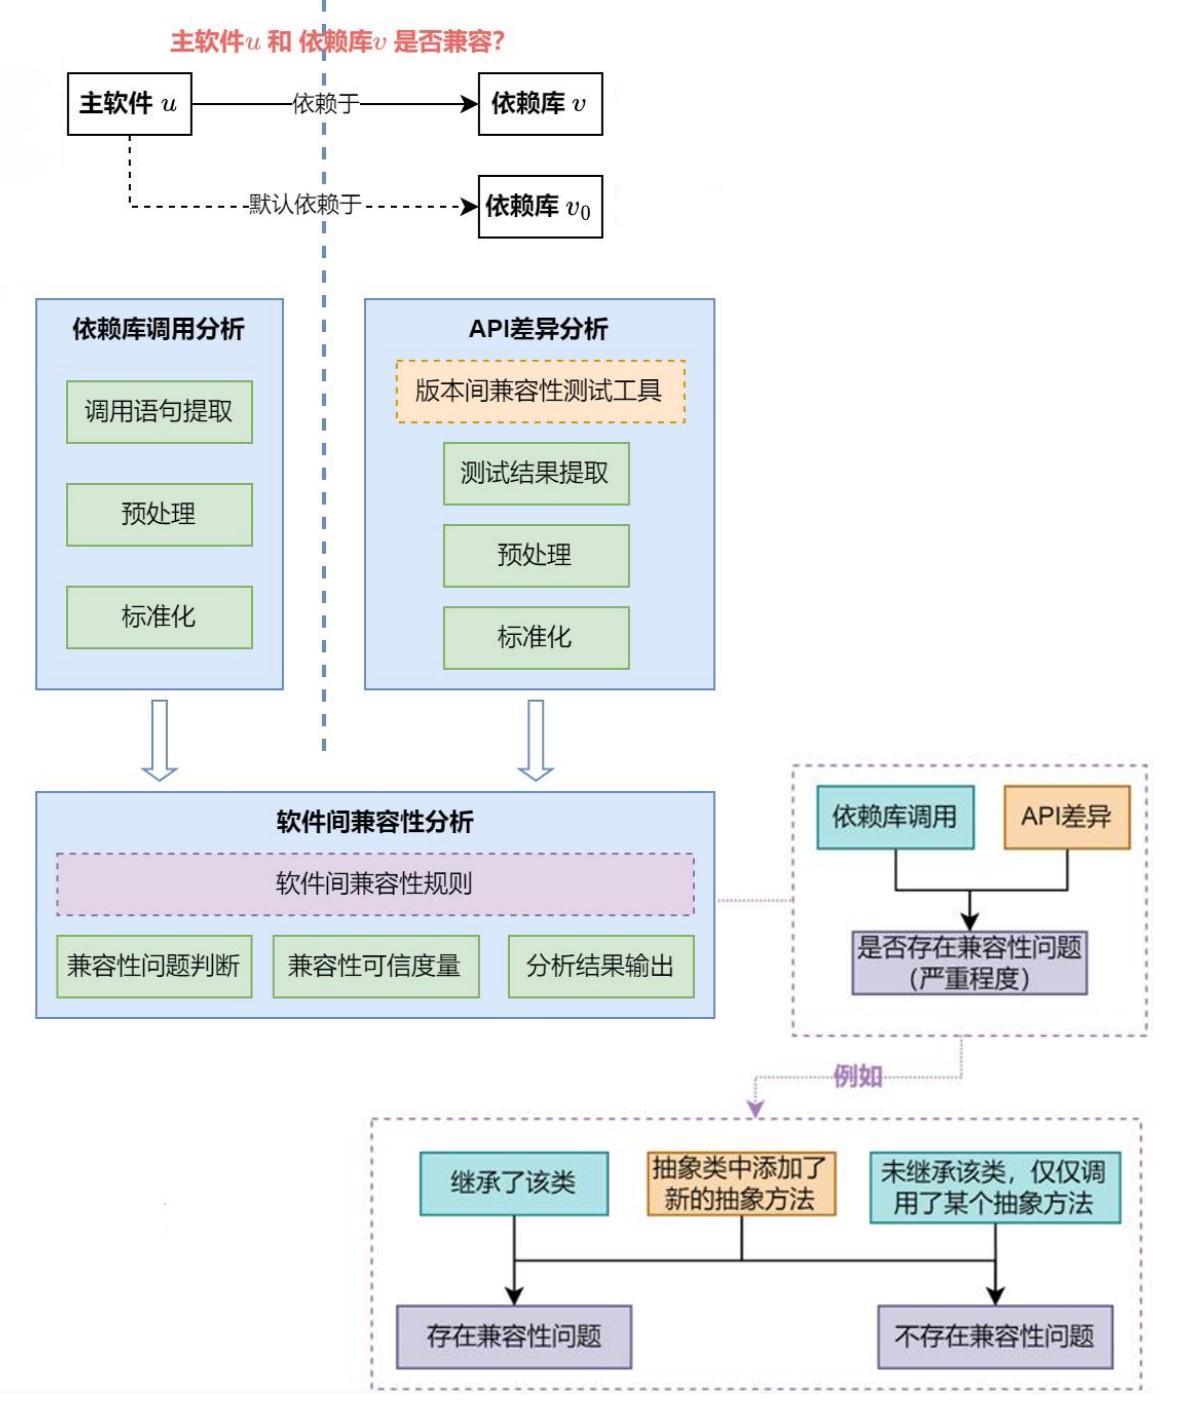
\includegraphics[width=0.5\textwidth]{img11/final.png}
    \label{fig:compatibility_test_framework}
\end{figure}

\begin{multicols}{3} % 分成两栏

    \subsection*{1. 依赖库调用分析}
    \begin{itemize}
        \item \textbf{任务}:提取主软件源代码中对依赖库的\textbf{API调用语句},以便分析主软件如何调用依赖库。
        \item \textbf{分析内容}:
        \begin{itemize}
            \item API类型(类、接口、方法等)
            \item 调用形式(类继承、方法调用、方法重载等)
        \end{itemize}
        \item \textbf{流程}:
        \begin{enumerate}
            \item 调用语句提取
            \item 数据预处理
            \item 数据标准化
        \end{enumerate}
    \end{itemize}
    
    \columnbreak % 在这里从中间分割
    
    \subsection*{2. API差异分析}
    \begin{itemize}
        \item \textbf{任务}:比较当前版本和默认版本依赖库的\textbf{API差异},识别API变更点。
        \item \textbf{分析内容}:
        \begin{itemize}
            \item API的\textbf{类移除}、\textbf{方法参数数量变化}、\textbf{返回值类型变化}等。
            \item 借助开源的版本兼容性测试工具进行分析。
        \end{itemize}
        \item \textbf{流程}:
        \begin{enumerate}
            \item 提取API差异结果
            \item 数据预处理与标准化
        \end{enumerate}
    \end{itemize}
    
    \columnbreak % 在这里从中间分割

    \subsection*{3. 软件间兼容性分析}
    \begin{itemize}
    \item \textbf{任务}:基于提取的API调用信息和API差异,评估API差异对主软件的\textbf{影响}。
    \item \textbf{分析内容}:
    \begin{itemize}
        \item 通过\textbf{软件间兼容性规则}判断是否存在兼容性问题。
        \item 评估兼容性问题的\textbf{严重程度}。
    \end{itemize}
    \item \textbf{流程}:
    \begin{enumerate}
        \item 兼容性问题判断
        \item 兼容性可行度量
        \item 分析结果输出
    \end{enumerate}
\end{itemize}

\end{multicols} % 结束分栏

\begin{multicols}{2} % 分为两栏

    % 左侧流程图
    \noindent\textbf{流程图:}
    \begin{center}
        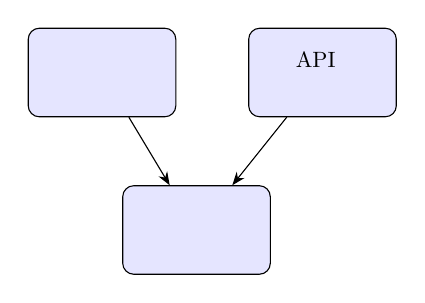
\begin{tikzpicture}[node distance=1cm, scale=0.8, transform shape]
            \tikzstyle{block} = [rectangle, draw, fill=blue!10, text width=6em, text centered, rounded corners, minimum height=4em]
            \tikzstyle{line} = [draw, -{Stealth}]
        
            % 定义节点
            \node[block] (start) {依赖库调 \\ 用分析};
            \node[block, right of=start, xshift=2.5cm] (api) {API 差 \\ 异分析};
            \node[block, below of=start, xshift=1.5cm, yshift=-1.5cm] (compatibility) {软件间兼容 \\ 性分析};
        
            % 添加箭头
            \path [line] (start) -- (compatibility);
            \path [line] (api) -- (compatibility);
        \end{tikzpicture}
    \end{center}
    
    \columnbreak % 分栏分隔符

    % 右侧简要分析信息
    \textbf{流程分析:}  

    主软件通过调用依赖库的 API,检测当前版本与默认版本之间的差异,评估这些差异是否引发兼容性问题。  

    \vspace{0.5cm}

    当直接依赖软件的某个抽象类中添加了新的抽象方法时,只有主软件继承了该类才会出现兼容性问题。
    
\end{multicols}

\newpage{}

\subsection{面向 Java 的工具平台框架}

\begin{figure}[H]
    \centering
    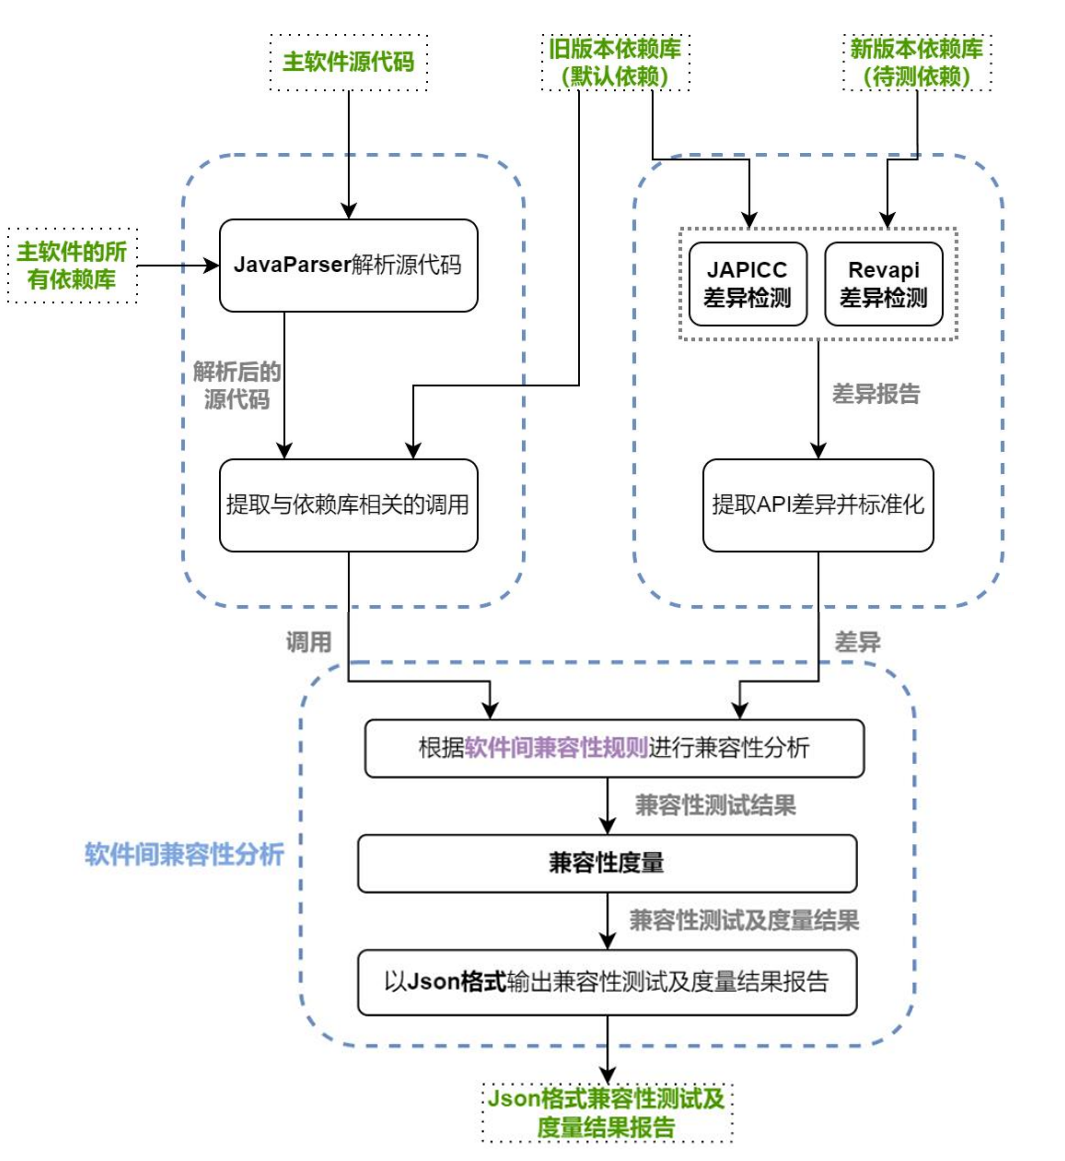
\includegraphics[width=0.48\textwidth]{img11/java.png}
    \label{fig:java}
\end{figure}

\begin{multicols}{3} % 分为三栏

    % 第一栏:解析主软件源代码
    \subsection*{1. 主软件解析与依赖提取}
    \begin{itemize}
        \item \textbf{任务}:解析主软件源代码,提取所有直接依赖的调用关系。
        \item \textbf{工具}:使用 \textbf{JavaParser} 工具对主软件源代码进行语法解析。
        \item \textbf{流程}:
        \begin{enumerate}
            \item 主软件的所有依赖库收集。
            \item 使用 JavaParser 解析源代码。
            \item 提取与依赖库相关的 API 调用语句。
        \end{enumerate}
    \end{itemize}

    \columnbreak % 分隔栏

    % 第二栏:API差异检测与标准化
    \subsection*{2. API 差异检测与标准化}
    \begin{itemize}
        \item \textbf{任务}:检测旧版本与新版本依赖库的 API 差异,并对差异进行标准化处理。
        \item \textbf{工具}:
        \begin{itemize}
            \item \textbf{JAPICC}:用于检测接口层面的 API 差异。
            \item \textbf{Revapi}:用于检测 API 变更的详细差异。
        \end{itemize}
        \item \textbf{流程}:
        \begin{enumerate}
            \item 比较旧版本(默认依赖)和新版本(待测依赖)的 API。
            \item 生成差异报告。
            \item 对差异报告进行标准化处理。
        \end{enumerate}
    \end{itemize}

    \columnbreak % 分隔栏

    % 第三栏:兼容性分析与结果输出
    \subsection*{3. 兼容性分析与结果输出}
    \begin{itemize}
        \item \textbf{任务}:基于差异报告和兼容性规则,分析兼容性问题,并输出结果。
        \item \textbf{实现}:
        \begin{itemize}
            \item 根据 \textbf{软件间兼容性规则} 进行兼容性分析。
            \item 计算 \textbf{兼容性度量},评估兼容性问题的严重程度。
        \end{itemize}
        \item \textbf{输出}:
        \begin{itemize}
            \item 生成兼容性测试和度量结果。
            \item 以 \textbf{JSON 格式} 输出最终结果报告。
        \end{itemize}
    \end{itemize}

\end{multicols}

\begin{multicols}{2} % 分为两栏

    \begin{center}
        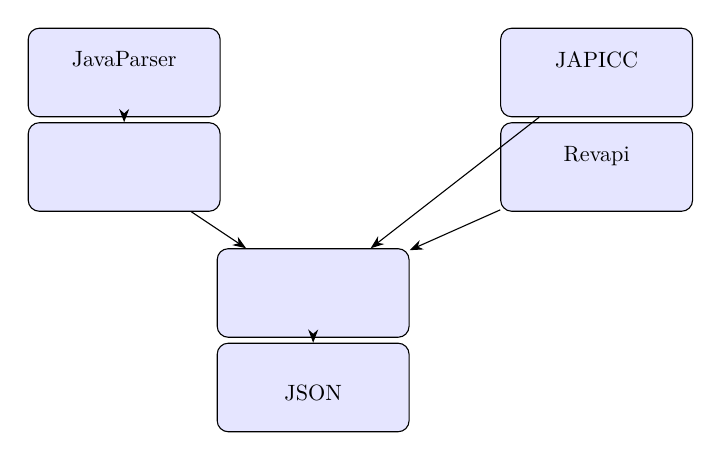
\begin{tikzpicture}[node distance=1.5cm, scale=0.8, transform shape]
            \tikzstyle{block} = [rectangle, draw, fill=blue!10, text width=8em, text centered, rounded corners, minimum height=4em]
            \tikzstyle{line} = [draw, -{Stealth}]
        
            % 定义节点
            \node[block] (parser) {JavaParser \\ 解析源代码};
            \node[block, below of=parser] (extract) {提取与依赖库相关的调用};
            \node[block, right of=parser, xshift=6cm] (japicc) {JAPICC \\ 差异检测};
            \node[block, below of=japicc] (revapi) {Revapi \\ 差异检测};
    
            % 中间节点 - 移动到中心
            \node[block, below of=extract, xshift=3cm, yshift=-0.5cm] (compat) {根据规则进行 \\ 兼容性分析};
            \node[block, below of=compat] (output) {兼容性度量 \\ 输出JSON报告};
    
            % 添加箭头
            \path [line] (parser) -- (extract);
            \path [line] (japicc) -- (compat);
            \path [line] (revapi) -- (compat);
            \path [line] (extract) -- (compat);
            \path [line] (compat) -- (output);
        \end{tikzpicture}
    \end{center}
    
    \columnbreak % 分栏分隔符

    % 右侧简要分析信息
    \noindent\textbf{流程分析:}  
    \begin{itemize}
        \item JavaParser 解析主软件源码,提取对依赖库的调用。  
        \item 通过工具检测新旧版本依赖库之间的 API 差异。  
        \item 基于兼容性规则分析差异的影响,度量兼容性问题,并输出 JSON 格式的结果报告。  
    \end{itemize}

    \noindent\textbf{注意事项:}
    当一个API调用受到多个API差异的影响时,受到影响的严重程度取高值。
    \[
    \textbf{High > Medium > Low > No}
    \]

\end{multicols}

\subsection{面向 Cpp 的工具平台框架}

\begin{figure}[H]
    \centering
        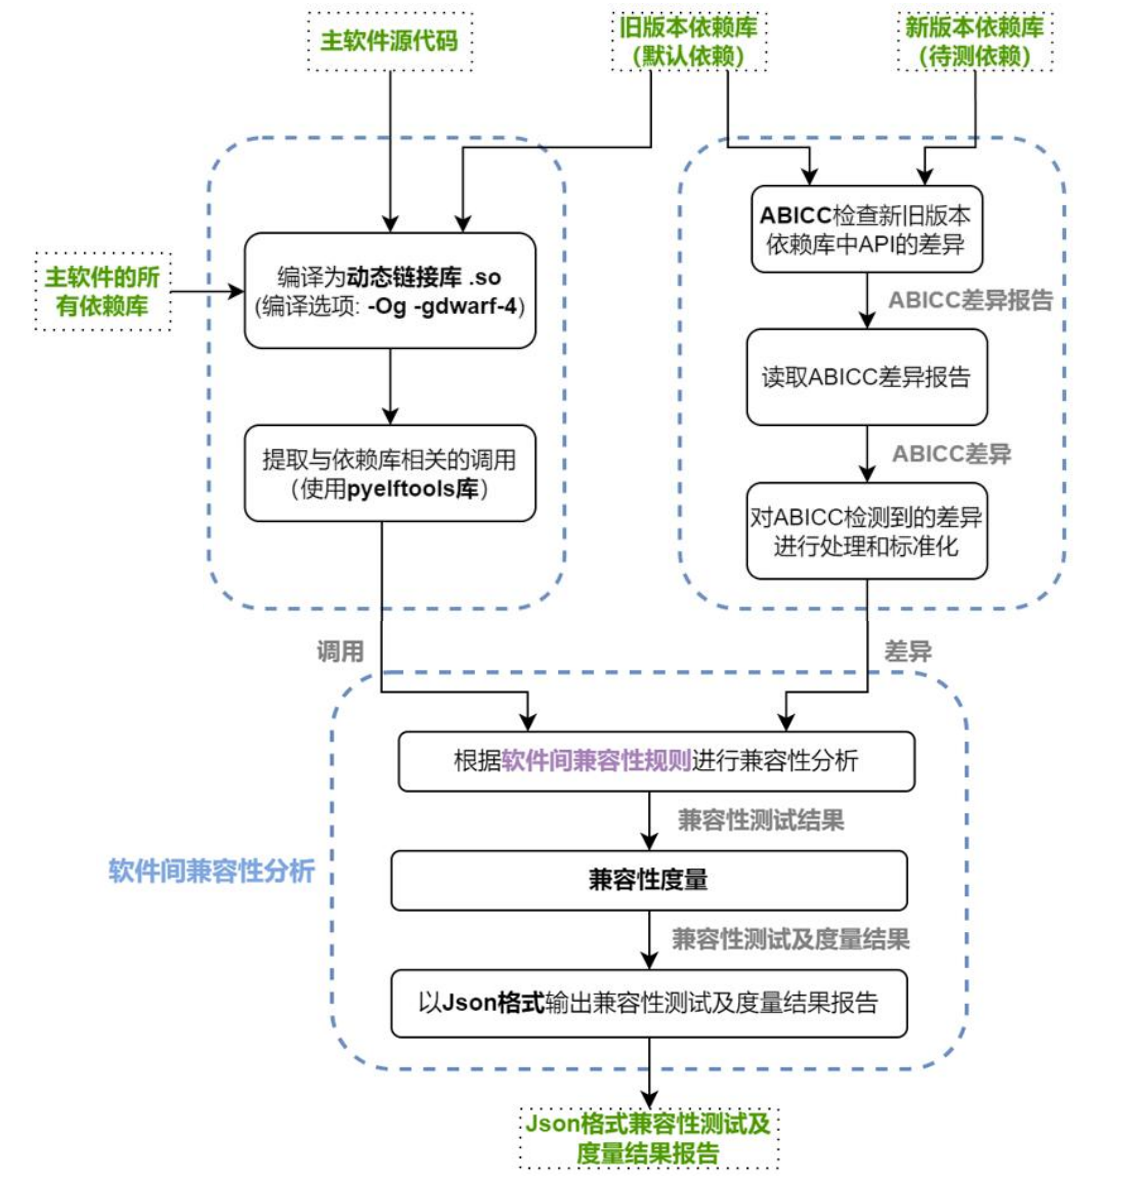
\includegraphics[width=0.4\textwidth]{img11/cpp.png}
        \label{fig:cpp} 
\end{figure}

\begin{multicols}{3} % 分为三栏

    % 第一栏:依赖库调用分析
    \subsection*{1. 依赖库调用分析}
    \begin{itemize}
        \item \textbf{任务}:编译主软件源代码,提取依赖库相关的 API 调用信息。
        \item \textbf{工具}:
        \begin{itemize}
            \item 编译工具链:生成动态链接库。
            \item \textbf{pyelftools}:读取调试信息,提取调用关系。
        \end{itemize}
        \item \textbf{流程}:
        \begin{enumerate}
            \item 编译源代码,保留调试信息。
            \item 使用 \textbf{pyelftools} 提取依赖库的调用信息。
        \end{enumerate}
    \end{itemize}

    \columnbreak % 分隔栏

    % 第二栏:API差异分析
    \subsection*{2. API 差异分析}
    \begin{itemize}
        \item \textbf{任务}:检测新旧版本依赖库的 API 差异,并标准化处理差异信息。
        \item \textbf{工具}:\textbf{ABICC}:检测 API 变更及差异。
        \item \textbf{流程}:
        \begin{enumerate}
            \item 使用 \textbf{ABICC} 检查当前版本和默认版本的 API 差异。
            \item 读取并解析差异报告。
            \item 对差异报告进行标准化处理,确保数据一致性。
        \end{enumerate}
    \end{itemize}

    \columnbreak % 分隔栏

    % 第三栏:兼容性分析与结果输出
    \subsection*{3. 兼容性分析与结果输出}
    \begin{itemize}
        \item \textbf{任务}:基于 API 差异和规则分析兼容性问题,生成兼容性度量报告。
        \item \textbf{实现}:
        \begin{itemize}
            \item 应用 \textbf{C/C++ 软件间兼容性规则} 分析 API 调用的影响。
            \item 确定兼容性影响的严重程度 (\textbf{High > Medium > Low > No})。
        \end{itemize}
        \item \textbf{输出}:
        \begin{itemize}
            \item 计算并生成兼容性测试与度量结果。
            \item 以 \textbf{JSON 格式} 输出最终结果报告,便于进一步分析。
        \end{itemize}
    \end{itemize}

\end{multicols}

\begin{multicols}{2}
    % 左侧流程图
    \begin{center}
        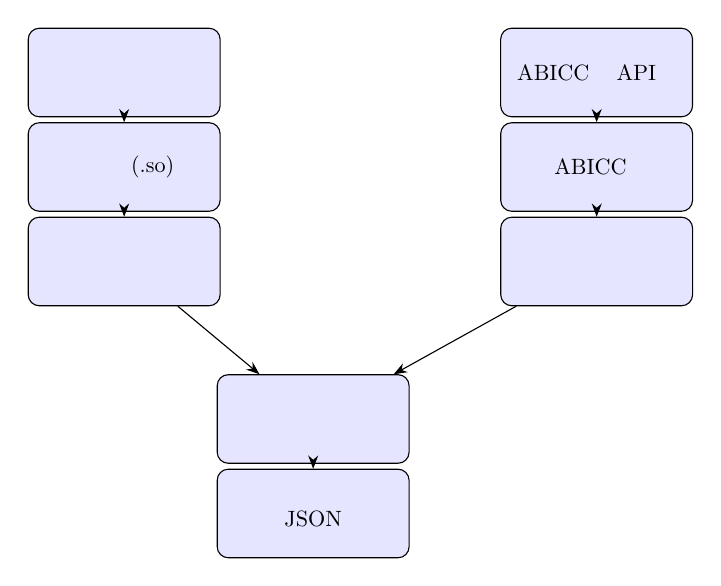
\begin{tikzpicture}[node distance=1.5cm, scale=0.8, transform shape]
            \tikzstyle{block} = [rectangle, draw, fill=blue!10, text width=8em, text centered, rounded corners, minimum height=4em]
            \tikzstyle{line} = [draw, -{Stealth}]
    
            % 定义节点
            \node[block] (source) {主软件源代码};
            \node[block, below of=source] (compile) {编译为动态链接库 (.so)};
            \node[block, below of=compile] (pyelf) {提取与依赖库相关的调用};
            
            \node[block, right of=source, xshift=6cm] (abicc1) {ABICC 检查 API 差异};
            \node[block, below of=abicc1] (report) {读取 ABICC 差异报告};
            \node[block, below of=report] (process) {差异处理与标准化};
    
            \node[block, below of=pyelf, yshift=-1cm, xshift=3cm] (compat) {根据规则进行兼容性分析};
            \node[block, below of=compat] (output) {兼容性度量 \\ 输出 JSON 报告};
    
            % 添加箭头
            \path [line] (source) -- (compile);
            \path [line] (compile) -- (pyelf);
            \path [line] (abicc1) -- (report);
            \path [line] (report) -- (process);
            \path [line] (pyelf) -- (compat);
            \path [line] (process) -- (compat);
            \path [line] (compat) -- (output);
        \end{tikzpicture}
    \end{center}
    
    \columnbreak % 分栏分隔符
    
    % 右侧简要分析信息
    \noindent\textbf{流程分析:}  
    \begin{itemize}
        \item 编译主软件源代码,生成动态链接库,并保留调试信息。  
        \item 使用 \textbf{ABICC} 检测新旧版本依赖库的 API 差异,标准化差异报告。  
        \item 根据兼容性规则评估 API 差异影响,计算兼容性度量,输出 \textbf{JSON 格式} 报告。  
    \end{itemize}

    \noindent\textbf{注意事项:}  
    当一个 API 调用受到多个差异的影响时,取最高严重程度:  
    \[
    \textbf{High > Medium > Low > No}
    \]

\end{multicols}

\end{document}